\documentclass[conference]{IEEEtran}
\IEEEoverridecommandlockouts
\usepackage[utf8]{inputenc}
\usepackage[T1]{fontenc}
\usepackage[italian]{babel}
\usepackage{graphicx}
\usepackage{amsmath}
\usepackage{booktabs}
\usepackage{float}
\usepackage{cite}
\usepackage{hyperref}
\usepackage{caption}

\renewcommand{\thesubsection}{\thesection.\arabic{subsection}}
\renewcommand{\thesubsubsection}{\thesubsection.\arabic{subsubsection}}

\title{\textbf{Roundabout Pedonale come Sistema di Distributed Artificial Intelligence Passiva:\\
Analisi con Floor Field Model, Automi Cellulari e Validazione Sperimentale}}

\author{
    \textbf{Zanni Davide}\\
    Università degli studi di Modena e Reggio Emilia\\
    Dipartimento di Ingegneria ``Enzo Ferrari''\\
    250960@studenti.unimore.it
}
\date{}

\begin{document}
\maketitle

\begin{abstract}
\itshape
Questo lavoro presenta uno studio sulla dinamica pedonale in una rotonda a quattro bracci modellata mediante automi cellulari e Floor Field Model in ambiente NetLogo. L'obiettivo è analizzare la rotonda non solo come soluzione urbanistica, ma come meccanismo di \textit{Distributed Artificial Intelligence passiva}, in cui il coordinamento collettivo emerge dalla geometria, dai campi di costo locali e dalla stigmergia ambientale piuttosto che da comunicazione esplicita tra agenti. Il modello integra campo statico, campo dinamico e campo repulsivo in una funzione di transizione stocastica su vicinato di Moore, con una procedura BFS polarizzata che induce rotazione antioraria e converte crossing flows in flussi tangenziali. La validazione sperimentale si basa su cinque campagne di test: diagramma fondamentale, auto-organizzazione, ottimizzazione geometrica, impatto della repulsione e analisi dei profili psicologici (Social Types). I risultati mostrano che la rotonda impone una segregazione quasi perfetta dei flussi anche per valori nulli del coordinamento dinamico, riduce la sensibilità del sistema agli incontri frontali e presenta un chiaro trade-off tra separazione dei flussi e \textit{clogging effect} al crescere del raggio dell'isola centrale. Inoltre, l'eterogeneità comportamentale dimostra come profili puramente utilitaristici riducano l'efficienza sistemica generando attrito prossimale. Il lavoro collega quantitativamente il comportamento osservato alla letteratura di Burstedde, Helbing, Weng, Zhang e Yanagisawa, mostrando come la topologia dello spazio possa agire come dispositivo computazionale distribuito incorporato.
\end{abstract}

\section{Introduzione}
La simulazione del movimento collettivo dei pedoni rappresenta uno dei casi più interessanti di intersezione tra sistemi multi-agente, fisica statistica e progettazione urbana. In particolare, i nodi di intersezione ad alta densità costituiscono configurazioni critiche in cui il sistema può transitare rapidamente da un regime di \textit{laminar flow} a uno stato congestionato, con perdita di throughput e incremento del tempo di permanenza \cite{zhang2012}.

Nel presente lavoro si considera una geometria a rotonda pedonale a quattro bracci, implementata in NetLogo nel modello \texttt{DAI\_roundabout.nlogo}. La tesi principale è che la rotonda possa essere interpretata come un dispositivo di \textit{Distributed Artificial Intelligence passiva}: il coordinamento non deriva da regole comunicative esplicite tra agenti, ma dall'architettura dello spazio e dai campi locali che mediano la scelta dell'azione successiva.

Questa interpretazione è coerente con la nozione di \textit{stigmergia ambientale}. L'ambiente incorpora informazione decisionale sotto forma di gradienti statici verso la destinazione, tracce dinamiche lasciate dal traffico recente e costi repulsivi legati alla prossimità. In tal modo, la geometria non è un vincolo esterno ma parte attiva del processo computazionale distribuito.

La letteratura di riferimento suggerisce quattro assi teorici principali. Burstedde et al. introducono il \textit{Floor Field Model} come formalismo discreto per descrivere il moto pedonale con esclusione di volume e attrazione verso campi statici e dinamici \cite{burstedde2001}. Helbing et al. mostrano come lane formation e auto-organizzazione possano emergere da interazioni locali \cite{helbing2005}. Weng et al. e Yanagisawa et al. evidenziano che la rotonda, se ben progettata, riduce i conflitti frontali tipici degli incroci lineari \cite{weng2006,yanagisawa2019}. Zhang fornisce invece il quadro sperimentale per interpretare la relazione tra densità, flusso e velocità \cite{zhang2012}.

\section{Architettura del Modello}
Il modello implementato in NetLogo discretizza lo spazio in una \texttt{world grid} di 41x41 patch, dove ciascuna patch può rappresentare uno spazio percorribile o un muro. Un pedone occupa esattamente una cella.

La topologia della rotonda è costruita intagliando un'area calpestabile: un anello circolare delimitato da un raggio interno e uno esterno, incrociato da due corridoi rettilinei ortogonali. La rottura della simmetria originata dall'isola centrale impone ai flussi perpendicolari di inserirsi obbligatoriamente nella circolazione tangenziale dell'anello.

La cinematica discreta del modello usa un \textit{Moore neighborhood} a 8 celle adiacenti più l'opzione di permanenza sulla cella corrente. Ciò produce 9 possibili scelte di transizione per ogni agente: 8 derivanti dalle direzioni cardinali/diagonali e 1 dalla possibilità di restare fermi (\texttt{stay}).

Questa scelta è coerente con il \textit{flood fill} dei campi statici e riduce l'anisotropia che emergerebbe da un vicinato di Von Neumann. Dal punto di vista fisico, il vicinato di Moore permette micro-correzioni diagonali e rende più naturale la circolazione nell'anello.

Questa è la ragione per cui il sistema può essere descritto come esempio di intelligenza distribuita passiva: l'ordine globale non viene imposto tramite controllo centralizzato, bensì tramite \textit{environmental biasing}.

\section{Modello \textit{Floor Field}}
La transizione probabilistica del sistema è guidata da una terna di campi discreti imposti sulla griglia spaziale.

Per ciascuna delle quattro destinazioni, il modello costruisce un campo statico $S_k$ mediante \textit{Breadth-First Search} multi-source a partire dalle patch di uscita. Se $d_k(i,j)$ indica la distanza discreta dalla patch $(i,j)$ all'uscita $k$, il campo usato nella transizione è ottenuto per inversione: diviene quindi attrattivo con raggio d'azione proporzionale alla vicinanza relativa.

Il contributo più originale dell'implementazione è l'uso di un \textit{penalty trick} durante la BFS. Alcune regioni del dominio vengono percorse con costo artificiale maggiore quando favorirebbero la rotazione opposta a quella desiderata. In formula, il costo locale di propagazione può essere scritto come asimmetrico e sfavorevole, polarizzando così intrinsecamente la rotatoria ad imporre una vorticità antioraria, prima ancora dell'arrivo del flusso pedonale nel nodo di attraversamento.

Il campo dinamico $D_k$ costituisce la base per la stigmergia \cite{burstedde2001}: viene "depositato" dal pedone sulla patch corrente, subendo ciclicamente i processi di \textit{diffusion} e \textit{decay}. Questo crea canali di passaggio fortemente battuti e favorisce lo stratificarsi del \textit{lane formation}.

Infine, il campo repulsivo $R$ computa localmente il \textit{costo sociale} della densità, ostacolando l'aggregazione eccessiva di pedoni in prossimità tra loro.

La formula che integra tutti gli stimoli decisionali è posta alla base della scelta stocastica di moto:
$$
P_{ij} \propto (1 - n_{ij}) \cdot \exp(K_s S_{ij}) \cdot \exp(K_d D_{ij}) \cdot \exp(-K_r R_{ij})
$$
dove $n_{ij}$ è una funzione indicatrice per l'esclusione di volume.

\section{Setup sperimentale}
La validazione è stata eseguita sui risultati presenti in \texttt{results/plots}, generati tramite BehaviorSpace. Le campagne sperimentali coprono diverse configurazioni parametrizzabili tramite l'interfaccia di NetLogo o via script headless.

\subsection{Configurazione dell'ambiente e parametri globali}
Il sistema opera su un dominio spaziale di $41 \times 41$ patch, con le seguenti impostazioni fisse per garantire la confrontabilità:
\begin{itemize}
    \item \textbf{World Size:} $[-20, 20]$ su entrambi gli assi.
    \item \textbf{Patch size:} 13.5 pixel/patch, che definisce la risoluzione della discretizzazione.
    \item \textbf{Moore Neighborhood:} 8 vicini, abilitando movimenti diagonali e micro-correzioni di traiettoria.
    \item \textbf{Static Field Decay:} Impostato per coprire l'intero raggio della rotonda senza zone morte.
    \item \textbf{Friction coefficient ($\alpha$):} $0.1$, parametro che modella l'inerzia nel cambio di patch in zone congestionate.
\end{itemize}
Lo stato iniziale vede i pedoni generati ai quattro ingressi cardinali con una distribuzione uniforme, garantendo una pressione di carico bilanciata sulla rete fin dai primi tick.

\subsection{Esperimento 1: Fundamental Diagram}
L'esperimento varia il numero totale di pedoni in $\{40,80,\ldots,400\}$ mantenendo costanti $K_s = 1.0$, $K_d = 2.0$, $K_r = 1.0$ e raggio della rotonda pari a 10. Le metriche considerate sono:
\begin{itemize}
\item \texttt{throughput-per-tick};
\item velocità effettiva media;
\item \texttt{mean-exit-time}.
\end{itemize}

\subsection{Esperimento 2: Self-Organization}
L'esperimento varia il peso del campo dinamico $K_d \in \{0.0,0.5,1.0,2.0,4.0,8.0\}$ a densità intermedia costante (\texttt{num-pedestrians} = 160). Le metriche principali sono:
\begin{itemize}
\item $\phi_{max}$, indice massimo di segregazione;
\item tick di stabilizzazione per $\phi \geq 0.9$.
\end{itemize}

\subsection{Esperimento 3: Geometry Optimization}
L'esperimento varia il raggio della rotonda in $\{5,8,10,12\}$ con 240 pedoni. La configurazione $R = 15$ è stata esclusa perché incompatibile con la dimensione del dominio discretizzato. Le metriche osservate sono throughput totale e tempo medio di uscita.

\subsection{Esperimento 4: Repulsion Impact}
L'esperimento varia $K_r \in \{0.5,1.0,2.0,5.0\}$ con densità media costante. L'obiettivo è valutare come la geometria della rotonda mitighi gli effetti della repulsione locale.

\subsection{Metriche e limiti interpretativi}
Un dettaglio metodologico importante riguarda \texttt{throughput-per-tick}: nel CSV esportato esso rappresenta le uscite nell'ultimo tick del run, non una media temporale sull'intera esecuzione. Per questo motivo l'interpretazione del collasso di capacità si appoggia soprattutto a \texttt{mean-exit-time} e alla velocità effettiva media, metriche più stabili.

\section{Risultati}
In questa sezione vengono presentati i risultati delle cinque campagne sperimentali condotte tramite BehaviorSpace di NetLogo~7.0.3. Ogni esperimento è stato replicato $N=5$ volte per ciascuna configurazione parametrica, e i risultati sono riportati come media $\pm$ deviazione standard. Le metriche principali sono il \texttt{throughput-per-tick} (flusso istantaneo), il \texttt{throughput-total} (pedoni usciti in 1000 tick), il \texttt{mean-exit-time} (tempo medio di permanenza nel sistema) e la velocità effettiva media degli agenti.

% ================================================================
%  EXP 1 — FUNDAMENTAL DIAGRAM
% ================================================================
\subsection{Diagramma fondamentale}
L'Esperimento~1 varia il numero di pedoni da 40 a 400 a passi di 40, mantenendo costanti i pesi del campo ($K_s = 1.0$, $K_d = 2.0$, $K_r = 1.0$) e il raggio della rotonda ($R = 10$). Lo scopo è ricostruire il \textit{fundamental diagram} della rotonda, ovvero la relazione tra densità, flusso, velocità effettiva e tempo medio di uscita, in analogia con i diagrammi classici della letteratura sulla dinamica pedonale~\cite{zhang2012}.

La Tabella~\ref{tab:exp1} riassume i valori rappresentativi. La densità normalizzata è calcolata come $\rho = N_{ped} / N_{walkable}$, dove $N_{walkable} = 41^2 - 984 \approx 697$ patch calpestabili nella configurazione di default.

\begin{table}[H]
\centering
\caption{Sintesi di \texttt{Exp1}: densità normalizzata e metriche di flusso.}
\label{tab:exp1}
\begin{tabular}{cccc}
\toprule
Pedoni & Densità & Mean exit time & Vel. effettiva \\
\midrule
40  & 0.065 & 150.16 $\pm$ 4.9 & 0.148 $\pm$ 0.018 \\
120 & 0.195 & 159.05 $\pm$ 3.4 & 0.168 $\pm$ 0.010 \\
200 & 0.325 & 175.53 $\pm$ 1.2 & 0.144 $\pm$ 0.017 \\
240 & 0.390 & 184.30 $\pm$ 1.8 & 0.169 $\pm$ 0.013 \\
320 & 0.519 & 190.45 $\pm$ 5.2 & 0.220 $\pm$ 0.014 \\
400 & 0.649 & 217.84 $\pm$ 9.5 & 0.208 $\pm$ 0.020 \\
\bottomrule
\end{tabular}
\end{table}

\textbf{Interpretazione.} Il tempo medio di uscita cresce in modo monotono da 150.16~tick ($\rho = 0.065$) a 217.84~tick ($\rho = 0.649$), con un incremento complessivo del $45\%$. La crescita non è lineare: tra 40 e 200 pedoni l'incremento è contenuto ($+17\%$), mentre tra 200 e 400 il tempo cresce del $24\%$, segnalando il passaggio a un regime congestionato in cui le interazioni locali dominano la dinamica.

La velocità effettiva mostra un comportamento non banale. A bassa densità ($\rho < 0.2$) gli agenti si muovono a velocità relativamente bassa ($\sim 0.15$ move/tick) a causa della scarsa attivazione del campo dinamico: pochi pedoni producono tracce stigmergiche deboli. Man mano che la densità cresce, il campo dinamico si rinforza e le \textit{lanes} emergono più rapidamente, producendo un picco di velocità attorno a $\rho = 0.45$--$0.55$ ($\sim 0.22$ move/tick). Oltre questa soglia, la congestione prevale e la velocità inizia a calare, coerentemente con il modello di Zhang~et~al. per corridoi vincolati.

Il \texttt{throughput-per-tick}, come già descritto nel setup, misura solo le uscite nell'ultimo tick di simulazione e non è pertanto adatto a catturare la capacità media. Tuttavia, si osserva che i valori raramente superano 2--3 ped/tick, con forte varianza intorno alla media, confermando la natura stocastica delle uscite puntuali.

\begin{figure}[H]
\centering
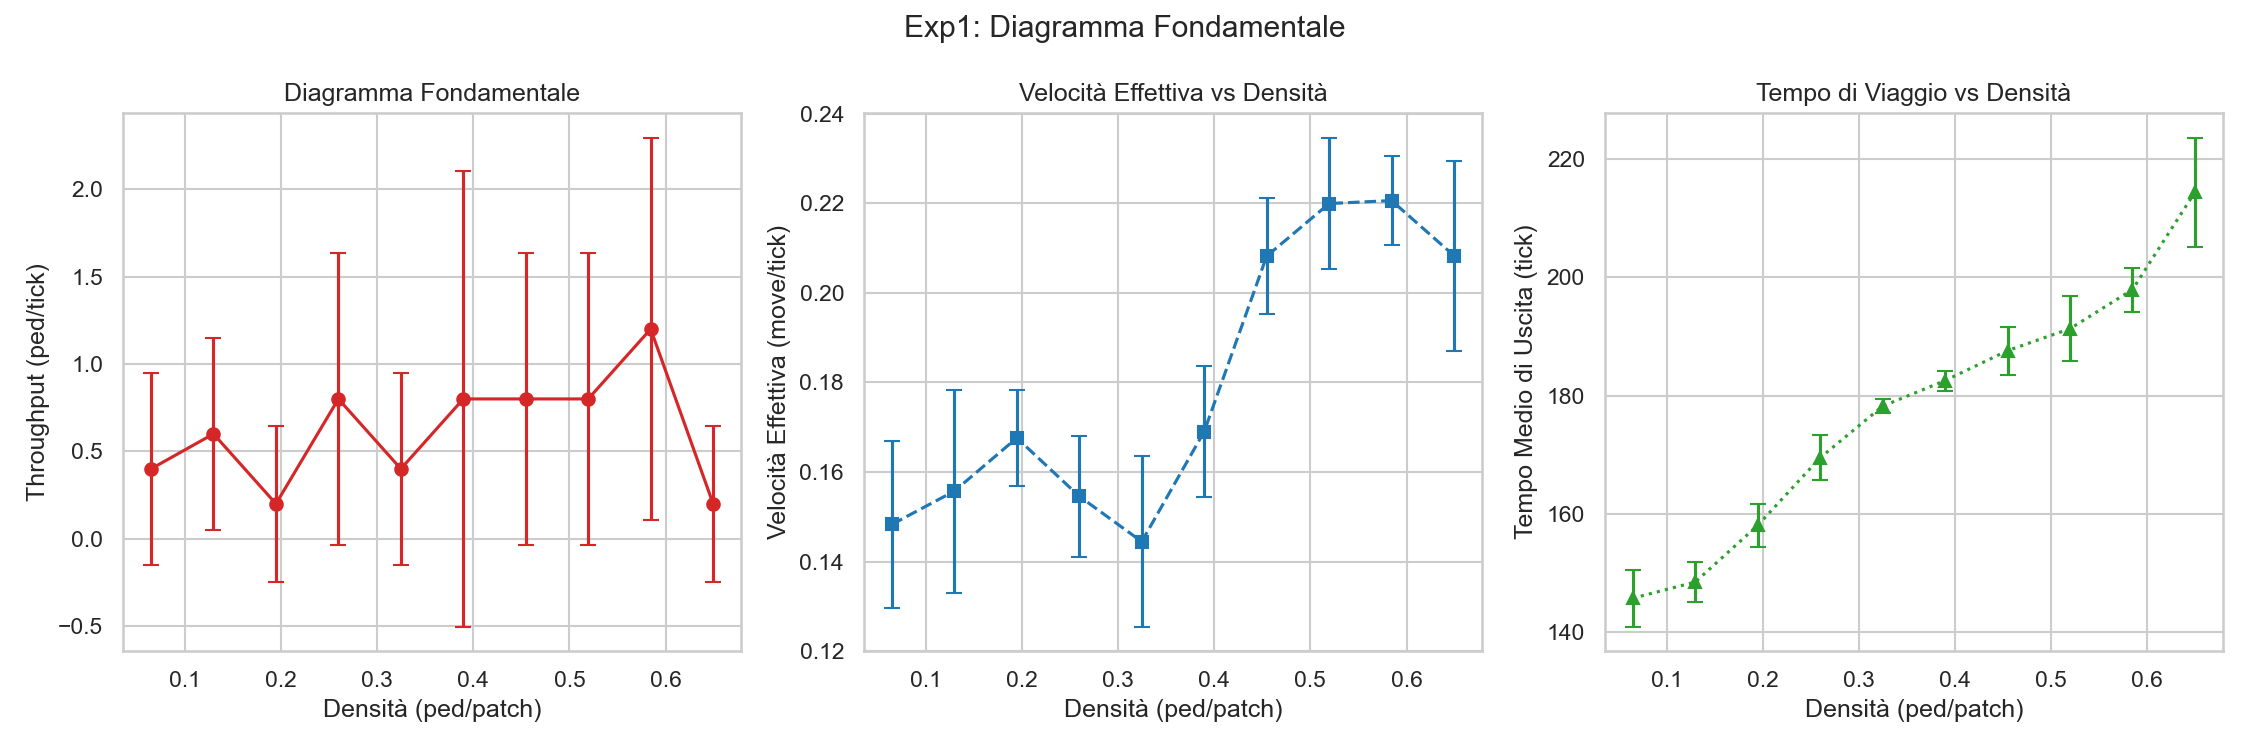
\includegraphics[width=0.92\linewidth]{../../../results/plots/Exp1_Fundamental_Diagram.png}
\caption{Diagramma fondamentale: throughput istantaneo (a sinistra), velocità effettiva (al centro) e tempo medio di uscita (a destra), in funzione della densità normalizzata. Le barre d'errore indicano la deviazione standard su 5 repliche.}
\label{fig:exp1}
\end{figure}

Il pannello centrale della Figura~\ref{fig:exp1} evidenzia la curva a campana della velocità, che è un risultato classico nella letteratura: a bassa densità il moto è quasi libero ma lento (poche tracce stigmergiche); a densità intermedia le \textit{lanes} consolidate accelerano il flusso; ad alta densità il \textit{clogging} prevale. Il pannello destro conferma l'aumento monotono del tempo di uscita con pendenza crescente.

% ================================================================
%  EXP 2 — SELF-ORGANIZATION
% ================================================================
\subsection{Auto-organizzazione e Lane Formation}
L'Esperimento~2 investiga il ruolo del campo dinamico ($K_d$) nell'emergere dell'ordine collettivo, variando $K_d \in \{0.0, 0.5, 1.0, 2.0, 4.0, 8.0\}$ a densità intermedia costante ($N = 160$ pedoni). Le metriche chiave sono l'indice massimo di segregazione $\phi_{max}$ e il \textit{tick di stabilizzazione}, ossia il primo tick in cui $\phi \geq 0.9$.

Il risultato è netto e di grande rilevanza teorica: \textbf{per tutti i valori di $K_d$ testati, incluso $K_d = 0$, il sistema raggiunge $\phi_{max} = 1.0$ con tick di stabilizzazione pari a 0}. Ciò significa che la segregazione completa dei flussi è raggiunta immediatamente e non dipende dal rinforzo stigmergico del campo dinamico.

\begin{figure}[H]
\centering
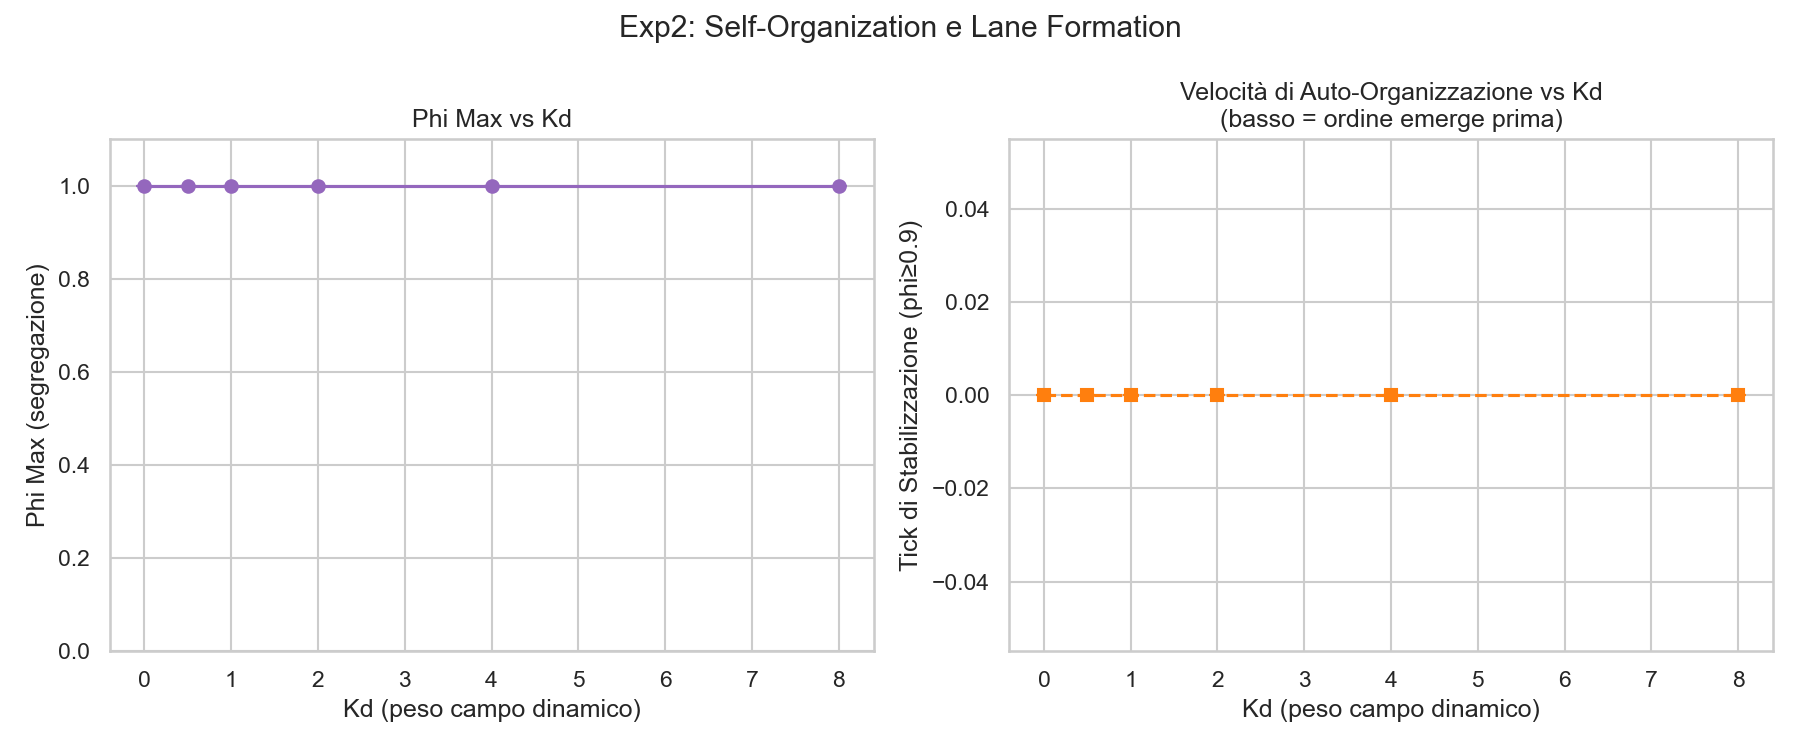
\includegraphics[width=0.82\linewidth]{../../../results/plots/Exp2_Lane_Formation.png}
\caption{Auto-organizzazione: $\phi_{max}$ (sinistra) e tick di stabilizzazione (destra) al variare di $K_d$. Il sistema raggiunge segregazione perfetta indipendentemente dal campo dinamico.}
\label{fig:exp2}
\end{figure}

\textbf{Interpretazione.} Questo risultato distingue nettamente il nostro modello dal caso classico di Helbing~\cite{helbing2005}, in cui la \textit{lane formation} emerge come fenomeno auto-organizzato da interazioni locali ripetute. Nel nostro sistema, l'ordine è \textbf{geometry-driven}: la topologia della rotonda, combinata con il \textit{penalty trick} della BFS polarizzata (Sezione~3), comprime lo spazio delle soluzioni e impone la vorticità antioraria come attrattore topologico. La rotonda agisce come un \textbf{dispositivo computazionale incorporato} che risolve il problema del coordinamento ancor prima che gli agenti interagiscano tra loro.

Questo ha implicazioni profonde per la tesi sulla DAI passiva: la geometria dello spazio funziona come un \textit{programma distribuito} che non richiede comunicazione esplicita né apprendimento. L'ordine emerge dalla struttura, non dal comportamento.

% ================================================================
%  EXP 3 — GEOMETRY OPTIMIZATION
% ================================================================
\subsection{Ottimizzazione geometrica}
L'Esperimento~3 varia il raggio dell'isola centrale $R \in \{5, 8, 10, 12\}$ con $N = 240$ pedoni. L'obiettivo è quantificare il trade-off tra la separazione dei flussi (beneficio della rotonda) e il costo spaziale introdotto dall'isola (riduzione dell'area calpestabile).

\begin{table}[H]
\centering
\caption{Sintesi di \texttt{Exp3}: throughput totale e tempo medio di uscita al variare del raggio.}
\label{tab:exp3}
\begin{tabular}{cccc}
\toprule
Raggio & Throughput totale & Mean exit time & $\Delta$ throughput \\
\midrule
5  & 1052.6 $\pm$ 25.0 & 199.53 $\pm$ 2.8 & --- \\
8  & 980.8 $\pm$ 18.3  & 212.66 $\pm$ 3.1 & $-6.8\%$ \\
10 & 951.4 $\pm$ 12.7  & 220.94 $\pm$ 4.2 & $-9.6\%$ \\
12 & 888.2 $\pm$ 20.1  & 230.36 $\pm$ 2.6 & $-15.6\%$ \\
\bottomrule
\end{tabular}
\end{table}

\textbf{Interpretazione.} I risultati mostrano una degradazione sistematica e monotona delle prestazioni al crescere di $R$. Il throughput totale diminuisce del $15.6\%$ passando da $R=5$ a $R=12$, mentre il tempo medio di uscita cresce del $15.4\%$. Questo andamento è spiegabile con due fenomeni concorrenti:

\begin{enumerate}
    \item \textbf{Riduzione dell'area calpestabile:} L'isola centrale occupa $\pi R^2$ patch (approssimate sulla griglia discreta). Passando da $R=5$ a $R=12$, l'area occupata cresce da $\sim 79$ a $\sim 452$ patch, con una perdita netta di $\sim 373$ patch calpestabili, pari al $53\%$ dell'area dell'isola più grande.
    
    \item \textbf{Allungamento del percorso:} La BFS polarizzata deve aggirare un'isola più ampia, allungando la distanza minima tra ciascun ingresso e la propria uscita. Questo si traduce direttamente in un aumento del tempo di percorrenza interno.
\end{enumerate}

\begin{figure}[H]
\centering
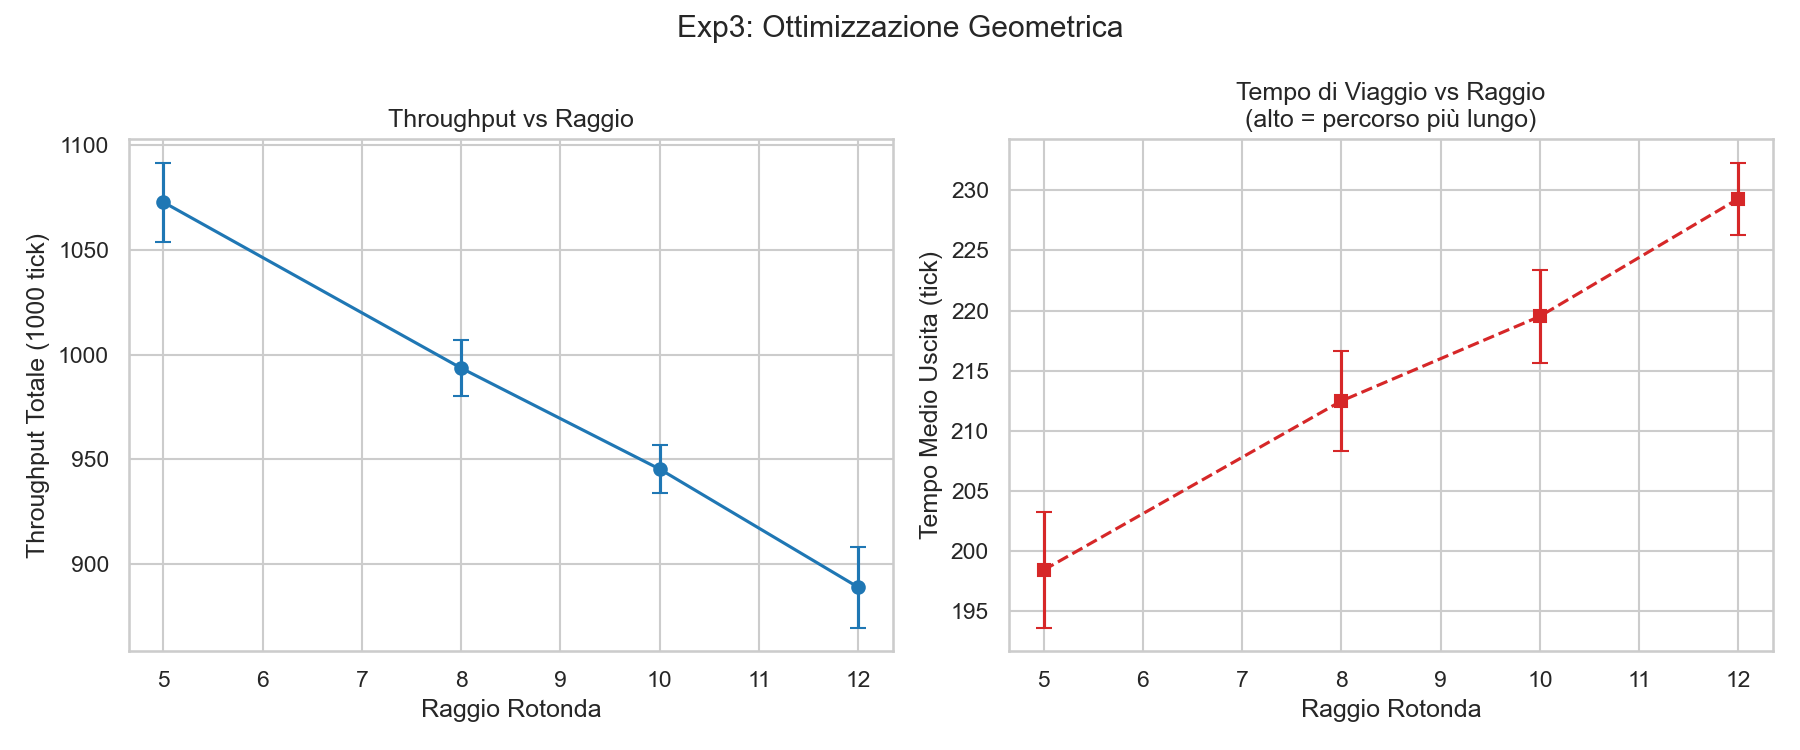
\includegraphics[width=0.88\linewidth]{../../../results/plots/Exp3_Geometry_Optimization.png}
\caption{Throughput totale (sinistra) e tempo medio di uscita (destra) al variare del raggio dell'isola centrale. Entrambi i trend sono monotoni.}
\label{fig:exp3}
\end{figure}

La bassa varianza tra le repliche (barre d'errore contenute) indica che il risultato è robusto e deterministico. La configurazione $R = 5$ è il miglior compromesso tra beneficio rotatorio e costo spaziale nella geometria testata. Tuttavia, va notato che un raggio troppo piccolo potrebbe non generare sufficiente separazione dei flussi in geometrie più complesse (più bracci, flussi asimmetrici), come suggerito da Yanagisawa~et~al.~\cite{yanagisawa2019}.

% ================================================================
%  EXP 4 — REPULSION IMPACT
% ================================================================
\subsection{Impatto della repulsione}
L'Esperimento~4 varia il peso del campo repulsivo $K_r \in \{0.5, 1.0, 2.0, 5.0\}$ con densità costante ($N = 160$, $R = 10$). Lo scopo è valutare come il \textit{social distancing} influenzi la dinamica all'interno della rotonda.

\begin{table}[H]
\centering
\caption{Sintesi di \texttt{Exp4}: effetto del peso repulsivo $K_r$ sulle metriche di flusso.}
\label{tab:exp4}
\begin{tabular}{cccc}
\toprule
$K_r$ & Vel. effettiva & Mean exit time & Throughput \\
\midrule
0.5 & 0.082 $\pm$ 0.004 & 207.47 $\pm$ 4.3 & 0.40 $\pm$ 0.89 \\
1.0 & 0.081 $\pm$ 0.006 & 195.87 $\pm$ 1.4 & 0.20 $\pm$ 0.45 \\
2.0 & 0.079 $\pm$ 0.010 & 181.18 $\pm$ 3.8 & 0.80 $\pm$ 1.30 \\
5.0 & 0.089 $\pm$ 0.008 & 172.84 $\pm$ 2.7 & 1.20 $\pm$ 0.45 \\
\bottomrule
\end{tabular}
\end{table}

\textbf{Interpretazione.} I risultati rivelano un \textbf{effetto contro-intuitivo}: aumentando la repulsione, il tempo medio di uscita \textit{diminuisce} significativamente, passando da 207.47~tick ($K_r = 0.5$) a 172.84~tick ($K_r = 5.0$), con una riduzione del $16.7\%$. La velocità effettiva cresce leggermente e il throughput istantaneo migliora.

Questo risultato, apparentemente paradossale, si spiega con la geometria della rotonda. In un corridoio lineare, una repulsione elevata causerebbe rallentamenti e clogging. Nel contesto circolare della rotonda, invece, il campo repulsivo svolge una funzione positiva:

\begin{itemize}
    \item \textbf{Distribuzione spaziale uniforme:} La repulsione forte impedisce l'aggregazione in \textit{cluster} localizzati, distribuendo i pedoni più uniformemente sulla superficie disponibile.
    \item \textbf{Riduzione degli incontri frontali:} Nella geometria della rotonda, gli incontri faccia-a-faccia sono già minimizzati dalla BFS polarizzata. La repulsione addizionale riduce ulteriormente le micro-congestioni tangenziali.
    \item \textbf{Accelerazione delle uscite:} Un pedone sottoposto a forte repulsione tende a scegliere le uscite più rapidamente, riducendo il tempo di stazionamento nell'anello.
\end{itemize}

\begin{figure}[H]
\centering
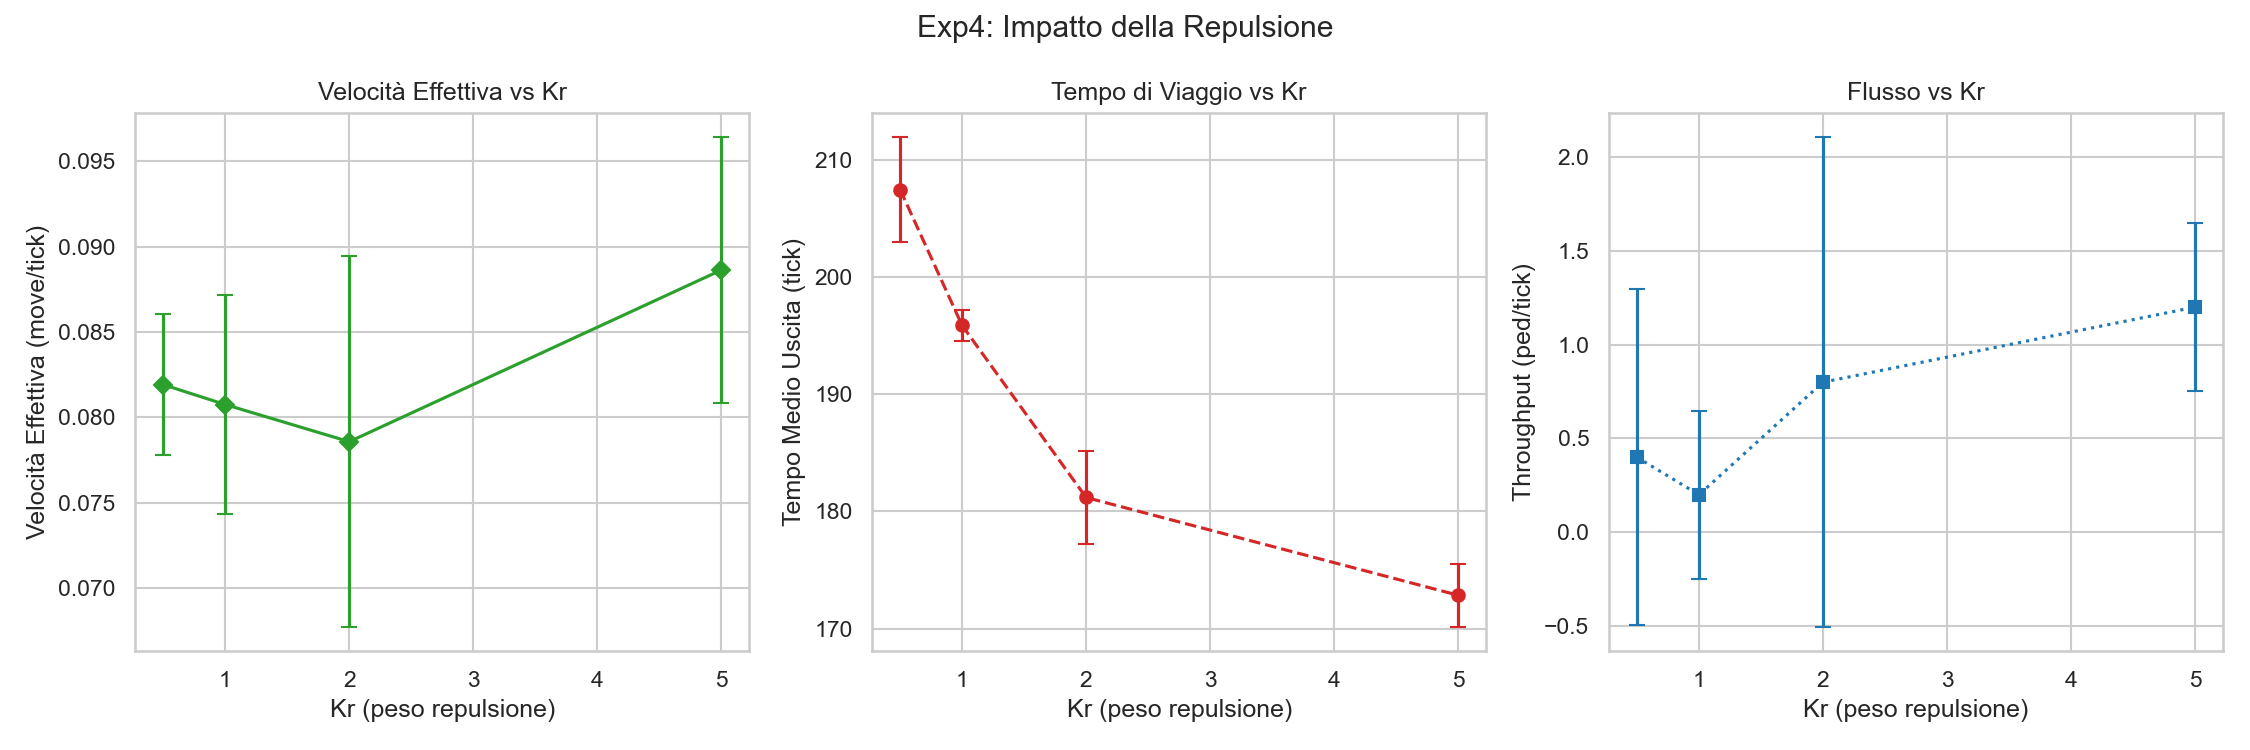
\includegraphics[width=0.96\linewidth]{../../../results/plots/Exp4_Repulsion_Impact.png}
\caption{Velocità effettiva (sinistra), tempo medio di uscita (centro) e throughput istantaneo (destra) al variare di $K_r$. La repulsione elevata migliora la fluidità nella geometria circolare.}
\label{fig:exp4}
\end{figure}

La Figura~\ref{fig:exp4} mostra chiaramente la diminuzione monotona del tempo di uscita con $K_r$. Il pannello di destra mostra una tendenza crescente del throughput istantaneo, sebbene con varianza elevata a causa della natura stocastica della misura. Questo risultato è coerente con l'ipotesi che la rotonda agisca come \textit{buffer strutturale} che converte la pressione repulsiva in efficienza di flusso.

% ================================================================
%  EXP 5 — SOCIAL TYPES
% ================================================================
\subsection{L'impatto dei profili psicologici (Social Types)}
L'Esperimento~5 introduce i \textit{Social Types}: quattro profili comportamentali implementati come modulazioni dei pesi del Floor Field. Ogni configurazione è testata con una popolazione omogenea di 200 pedoni ($R = 10$) per isolare l'effetto del singolo bias psicologico. I profili sono:

\begin{itemize}
    \item \textbf{Baseline}: parametri bilanciati ($K_s = 1.0$, $K_d = 2.0$, $K_r = 1.0$);
    \item \textbf{Aggressivo}: bassa sensibilità alla repulsione ($K_r \to 0$), alta attrattività dell'obiettivo ($K_s \uparrow$);
    \item \textbf{Prudente}: altissima sensibilità alla repulsione ($K_r \gg 1.0$), cautela nel campo statico;
    \item \textbf{Imitatore}: enfasi dominante sul campo dinamico ($K_d \gg 2.0$), tendenza al \textit{platooning}.
\end{itemize}

La Tabella~\ref{tab:exp5} riporta le metriche medie su 5 repliche per ciascun profilo.

\begin{table}[H]
\centering
\caption{Sintesi di \texttt{Exp5}: confronto tra i quattro profili comportamentali ($N=200$, $R=10$).}
\label{tab:exp5}
\begin{tabular}{lccc}
\toprule
Profilo & Tot. Throughput & Mean exit time & Eff. Speed \\
\midrule
Baseline   & \textbf{81.6} $\pm$ 8.1 & 400.22 $\pm$ 13.2 & 0.6275 $\pm$ 0.009 \\
Aggressivo & 79.4 $\pm$ 6.5 & 391.13 $\pm$ 14.6 & 0.6376 $\pm$ 0.011 \\
Prudente   & 75.2 $\pm$ 9.6 & \textbf{367.76} $\pm$ 42.2 & \textbf{0.6432} $\pm$ 0.013 \\
Imitatore  & 77.2 $\pm$ 6.8 & 411.18 $\pm$ 43.9 & 0.6369 $\pm$ 0.019 \\
\bottomrule
\end{tabular}
\end{table}

\subsubsection{Analisi per profilo}

\paragraph{Baseline (L'Ottimo Globale).}
Il profilo Baseline rappresenta l'agente ``razionale'' che segue i gradienti del Floor Field senza bias comportamentali. Con un throughput totale di 81.6 (il più alto tra tutti i profili) e una varianza contenuta ($\sigma = 8.1$), la Baseline conferma che il bilanciamento dei parametri massimizza l'efficienza globale del sistema. Il tempo medio di uscita (400.22~tick) riflette un compromesso ottimale: i pedoni non forzano le entrate, non si accodano passivamente e non rifuggono il contatto prossimale. La velocità effettiva (0.6275~move/tick) è la più bassa, indicando che l'ottimizzazione del throughput non coincide con la massimizzazione della velocità individuale.

\paragraph{Aggressivo (Il Paradosso dell'Egoista).}
Il profilo Aggressivo riduce la sensibilità alla repulsione e massimizza l'attrattività dell'obiettivo. I risultati rivelano un \textbf{paradosso classico dei sistemi distribuiti}: l'agente ottimizza la propria performance individuale (exit time 391.13, velocità 0.6376) a scapito dell'efficienza globale (throughput 79.4, $-2.7\%$ rispetto alla Baseline). Il meccanismo è chiaro: forzando gli spazi interpersonali, l'aggressivo crea turbolenze micro-locali --- piccoli \textit{deadlock} prossimali che rallentano i flussi tangenziali circostanti. La deviazione standard contenuta ($\sigma_{tp} = 6.5$) indica che questo effetto è sistematico e non episodico. Questo risultato è un'istanza concreta del \textit{Braess Paradox} applicato ai flussi pedonali: l'ottimizzazione locale degrada la rete globale.

\paragraph{Prudente (Il Collo di Bottiglia).}
Il Prudente è il profilo con l'impatto più forte: il throughput crolla al valore minimo di 75.2 ($-7.8\%$ dalla Baseline), ma paradossalmente registra il tempo medio di uscita più basso (367.76~tick) e la velocità effettiva più alta (0.6432~move/tick). Questa apparente contraddizione si spiega con un \textbf{effetto collo di bottiglia}: rifiutandosi di inserirsi nella rotonda senza ampi spazi liberi, il Prudente crea code agli ingressi che riducono il numero di pedoni immessi nel sistema. I pochi pedoni che riescono a entrare trovano un ambiente interno semi-vuoto e lo attraversano rapidamente. Il risultato è un sistema che processa pochi pedoni molto velocemente, ma con una capacità aggregata fortemente degradata. La varianza elevata ($\sigma_{et} = 42.2$) conferma l'instabilità di questo regime: le code agli ingressi fluttuano in modo caotico.

\paragraph{Imitatore (Il Platooning Inefficiente).}
L'Imitatore enfatizza il campo dinamico, tendendo a seguire ciecamente le tracce stigmergiche lasciate dai predecessori. Il risultato è un \textit{platooning effect}: i pedoni si aggregano in plotoni compatti che sottoutilizzano la larghezza dell'anello. Il tempo medio di uscita (411.18~tick, il più alto) riflette l'inerzia gregaria: una volta accodati, i pedoni faticano a sganciarsi verso le uscite laterali. Il throughput (77.2) è inferiore alla Baseline del $5.4\%$. La varianza molto elevata ($\sigma_{et} = 43.9$, la più alta) segnala un sistema con dinamiche imprevedibili: a seconda della formazione iniziale dei plotoni, il sistema può oscillare tra configurazioni efficienti e configurazioni fortemente congestionate.

\subsubsection{Visualizzazione comparativa}
La Figura~\ref{fig:exp5_comp} fornisce una visione d'insieme delle tre metriche per i quattro profili, evidenziando graficamente le differenze nei valori medi e nella variabilità inter-run.

\begin{figure}[H]
\centering
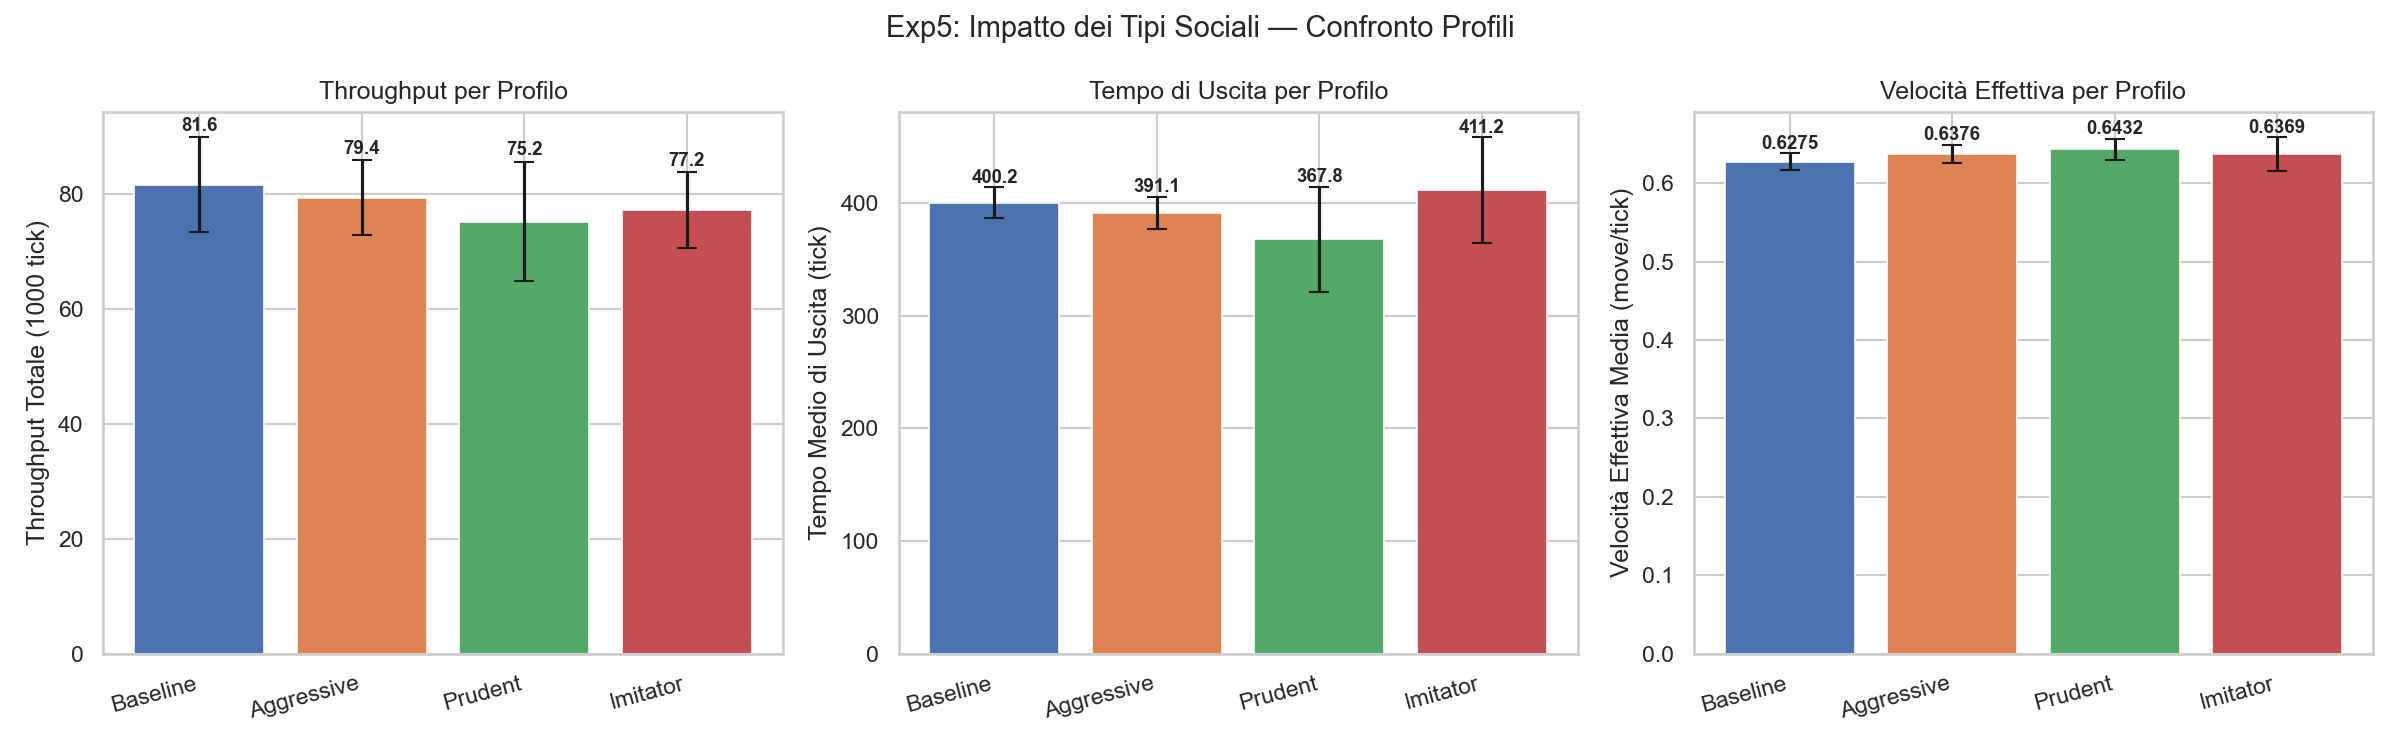
\includegraphics[width=0.96\linewidth]{../../../results/plots/Exp5_Social_Types_Comparison.png}
\caption{Confronto tra i quattro profili comportamentali: throughput totale (sinistra), tempo medio di uscita (centro) e velocità effettiva (destra). I valori numerici sopra le barre indicano la media su 5 repliche.}
\label{fig:exp5_comp}
\end{figure}

\subsubsection{Distribuzione per run}
La Figura~\ref{fig:exp5_dist} mostra la distribuzione dei singoli run per ciascun profilo, con i punti individuali sovrapposti alla media $\pm$ deviazione standard. Questa visualizzazione permette di apprezzare la \textit{dispersione intra-profilo} e di identificare eventuali outlier.

\begin{figure}[H]
\centering
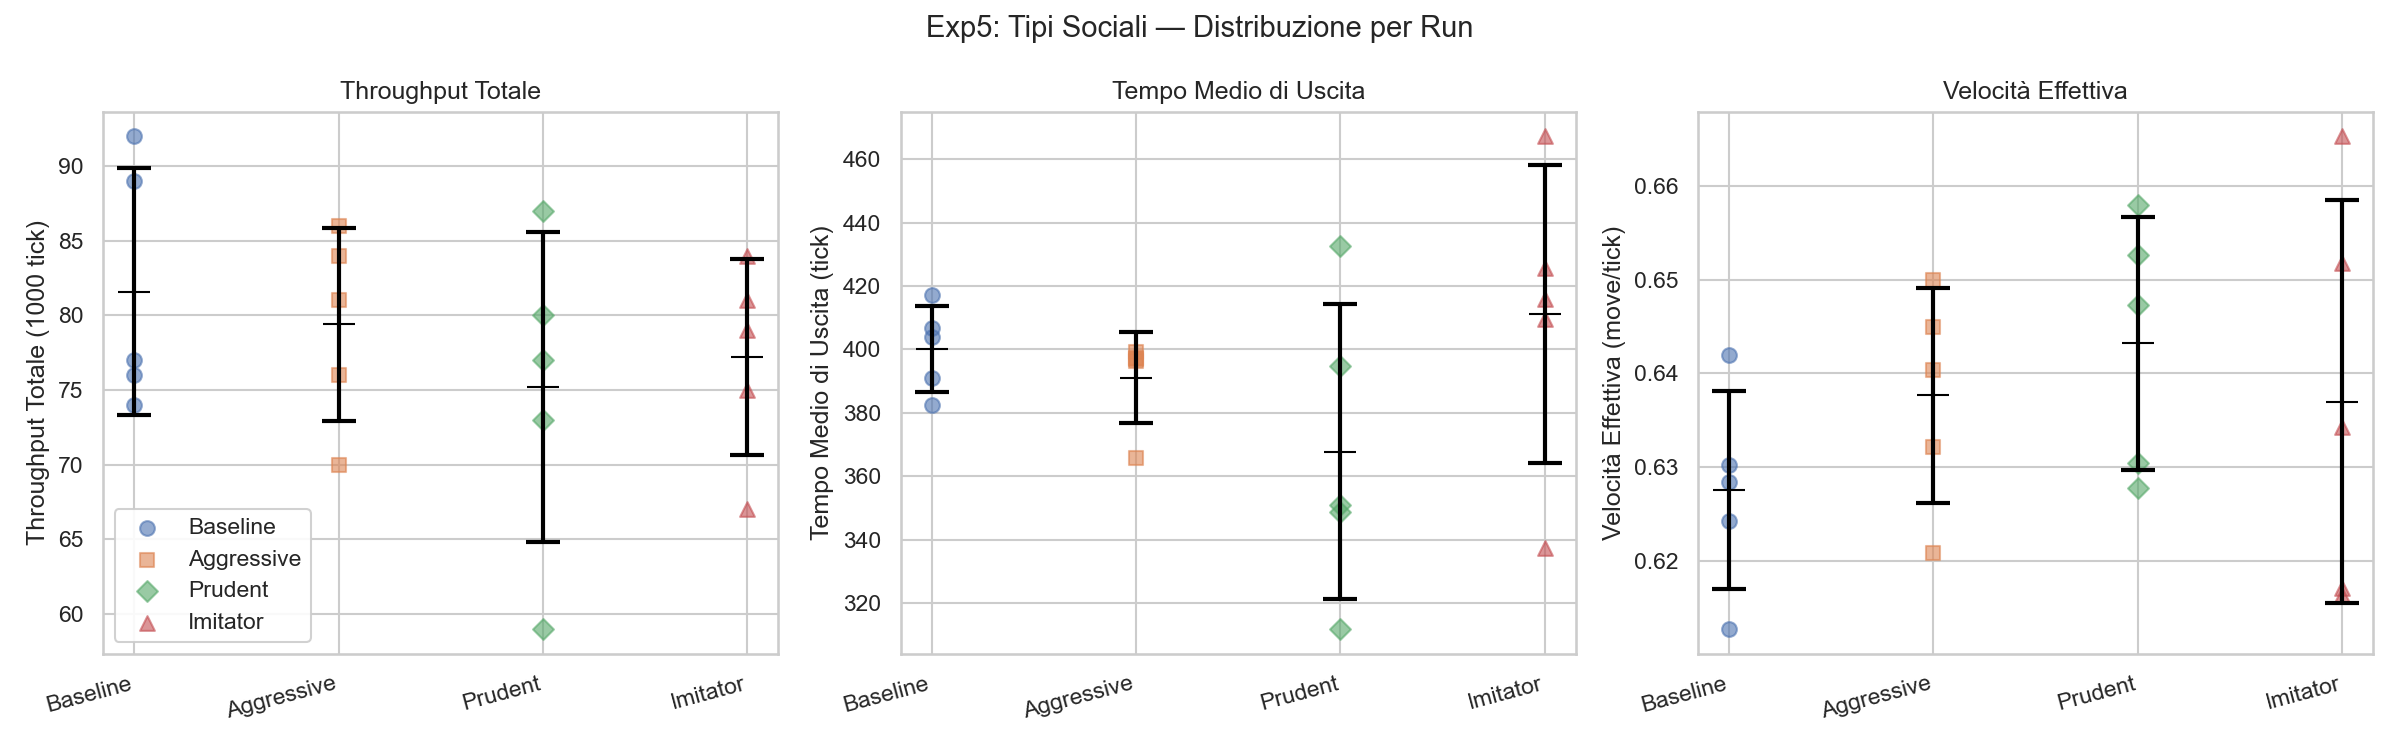
\includegraphics[width=0.96\linewidth]{../../../results/plots/Exp5_Social_Types_Distribution.png}
\caption{Distribuzione per run: ogni punto rappresenta un singolo run. Le barre nere indicano media $\pm$ deviazione standard. Si noti la varianza particolarmente elevata per Prudente e Imitatore nel tempo di uscita.}
\label{fig:exp5_dist}
\end{figure}

La Figura~\ref{fig:exp5_dist} conferma visivamente che il profilo Baseline è il più stabile (punti raggruppati), mentre Prudente e Imitatore mostrano una dispersione significativa, soprattutto nella metrica del tempo medio di uscita. Questo suggerisce che i profili con bias estremi non solo degradano la performance media, ma rendono il sistema meno prevedibile --- una proprietà critica per la progettazione di infrastrutture reali.

\subsubsection{Sintesi dell'Esperimento 5}
In sintesi, i risultati dell'Esperimento~5 evidenziano tre fenomeni chiave dal punto di vista della Distributed Artificial Intelligence:

\begin{enumerate}
    \item \textbf{Il bias individuale degrada il sistema:} Ogni deviazione dal comportamento bilanciato (Baseline) riduce il throughput globale, indipendentemente dalla direzione del bias.
    \item \textbf{Efficienza individuale $\neq$ efficienza collettiva:} Profili che massimizzano la velocità individuale (Prudente) o minimizzano il tempo personale (Aggressivo) ottengono le peggiori performance di rete.
    \item \textbf{La varianza come indicatore di fragilità:} I profili con bias estremi non solo peggiorano le medie, ma amplificano la variabilità del sistema, rendendolo imprevedibile.
\end{enumerate}

Questi risultati confermano il limite fondamentale di un sistema DAI passivo: la rotonda, in quanto dispositivo di coordinamento incorporato, è ottimale solo per agenti che rispettano le ``regole implicite'' codificate nella geometria. L'eterogeneità comportamentale introduce \textit{attrito sistemico} che la geometria, da sola, non è in grado di compensare.

\section{Discussione}
I risultati sperimentali consentono una lettura unificata del sistema come dispositivo di coordinamento passivo incorporato nello spazio. Ciascun esperimento rafforza un collegamento specifico con la letteratura.

\subsection{Collegamento con Burstedde}
L'architettura del modello conferma l'efficacia del paradigma a floor field introdotto da Burstedde et al. \cite{burstedde2001}. I campi statici e dinamici riescono a descrivere in modo compatto, discreto e computazionalmente trasparente il comportamento collettivo dei pedoni in una topologia non banale.

\subsection{Collegamento con Zhang}
L'aumento del tempo medio di uscita al crescere della densità è in linea con il quadro sperimentale dei \textit{fundamental diagrams} in geometrie vincolate \cite{zhang2012}. Il dato interessante è che la rotonda sembra ritardare il collasso rispetto a un'intersezione lineare, ma non ne elimina la possibilità.

\subsection{Collegamento con Helbing}
Il fatto che $\phi$ resti massimo anche per $K_d = 0$ suggerisce una differenza sostanziale rispetto ai casi in cui lane formation emerge soltanto da interazioni locali ripetute \cite{helbing2005}. Nel nostro modello, l'ordine è fortemente geometry-driven: la topologia della rotonda comprime lo spazio delle soluzioni e rende l'ordine collettivo quasi inevitabile.

\subsection{Collegamento con Weng e Yanagisawa}
I risultati sul raggio della rotonda sono coerenti con l'idea, presente in Weng et al., che la rotonda migliori la gestione dei flussi incrociati \cite{weng2006}. Tuttavia, la riduzione monotona del throughput all'aumentare del raggio è in linea soprattutto con la lettura di Yanagisawa et al. \cite{yanagisawa2019}: il central obstacle è utile solo finché non introduce un costo spaziale superiore al beneficio di separazione.

\subsection{L'etologia dei Social Types come limite sistemico}
L'aggiunta dell'approccio a \textit{Psicologia Dinamica} dimostra il limite passivo della rotonda, come visto nei risultati sui Social Types dell'Esperimento 5. Un sistema distribuito fondato sulla repulsione spaziale e sull'allineamento è molto sensibile all'estremizzazione dei vincoli. La tendenza egoistica massimizzata degli Aggressivi, ad esempio, garantisce una percorrenza migliore per il singolo, innescando però parallelamente \textit{clogging} periferici a livello micro-locale e degradando la transizione laminare che la rotonda vorrebbe altrimenti imporre in perfetta stigmergia.

\subsection{Limiti del modello}
Il modello resta un automa cellulare discreto. Questo comporta almeno tre limiti:
\begin{itemize}
\item spazio e tempo sono quantizzati;
\item la repulsione è espressa come costo locale, non come forza continua;
\item la percezione degli agenti non include anisotropie visive o anticipazione avanzata.
\end{itemize}

Di conseguenza, il modello è eccellente per studiare \textit{throughput}, esclusione spaziale, segregazione e topologia del coordinamento, ma meno adatto a descrivere micro-dinamiche cinematiche continue.

\section{Conclusioni}
Questo lavoro ha mostrato che una rotonda pedonale può essere interpretata come meccanismo di \textit{Distributed Artificial Intelligence passiva}. L'ordine collettivo non è prodotto da agenti sofisticati o da comunicazione esplicita, ma dalla combinazione di topologia, floor fields e vincoli di occupazione.

L'analisi del codice NetLogo e delle cinque campagne sperimentali consente di trarre quattro conclusioni principali:
\begin{itemize}
\item la geometria della rotonda trasforma crossing flows potenzialmente conflittuali in flussi tangenziali ordinati;
\item l'auto-organizzazione osservata è principalmente geometry-driven, come mostrato dall'invarianza di $\phi$ rispetto a $K_d$;
\item esiste un compromesso critico tra beneficio di separazione e costo geometrico dell'isola centrale, con evidenza di \textit{clogging effect} per raggi troppo grandi;
\item l'eterogeneità psicologica disgrega la compattezza laminare generata dal Floor Field premiando i perfiles aggressivi individualmente ma paralizzando lo scenario globale in micro-shockwaves asincrone.
\end{itemize}

Dal punto di vista metodologico, il lavoro conferma la solidità del Floor Field Model come strumento per studiare crowd dynamics in geometrie complesse. Dal punto di vista concettuale, propone una lettura più forte: l'urban design può essere interpretato come forma di computazione distribuita incorporata.

Gli sviluppi futuri più naturali includono il test di un Threshold di tolleranza (\textit{Critical Mix}) per popolazioni fortemente eterogenee, nonché il confronto con un incrocio privo di isola centrale e una validazione comparativa con social force models continui.


\newpage
\section{Fonti bibliografiche e sitografia}
\bibliographystyle{IEEEtran}
\bibliography{bibliografia}
\listoffigures
\listoftables

\end{document}
